%\section*{ Introduction to Repeated Two-person Zero-Sum Games}

%\markright{Rock-Paper-Scissors}
\section{Mixed Strategies: Graphical Solution}\index{graphical solution}

In this section we will learn a method for finding the maximin solution for a repeated game using a graph.

Let's continue to consider the game given in Example \ref{E:smallrepeat} by 

\[\left[\begin{matrix}
1&0\\
-1&2

\end{matrix}\right].\]

In order to make our analysis easier, let's name the row and column strategies as in Table \ref{T:smallrepeat}.

\begin{table}[h]
\centering
\begin{tabular}{rcc}
&\textbf{C}&\textbf{D}\\ 
\textbf{A} &1&0 \\ 
\textbf{B}&-1&2 \\ 
\end{tabular}
\caption{Example \ref{E:smallrepeat} with named strategies}
\label{T:smallrepeat}
\end{table}

We want to determine how often Player 1 should play A and how often she should play B.
\begin{xca}\label{E:linearconjecture}
First it is good to test your instinct. Do you think she should play one of the strategies more often than the other? If so, which strategy should she play the most?
\end{xca}

What we are really trying to find is the probability with which Player 1 plays A (or B). Since we know that the probabilities sum to one, if we can find one probability, then we know the other. 

Here is one way to do this. Let $p$ be the probability that Player 1 plays B. Let $m$ be the payoff to Player 1. Since we are try to find a mixed strategy for Player 1, we will pick a strategy for Player 2 and try to determine the possible payoffs for Player 1.

 Let us determine some pairs $(p, m)$.
\begin{itemize}
\item[Step 1.] Assume \textbf{Player 2} plays pure strategy \textbf{C}.
\begin{itemize}
\item[Step 1a.] Find the probability ($p$) and payoff ($m$) if Player 1 always plays \textbf{A}.

If Player 1 plays pure strategy A, then she never plays B. Thus the probability she plays B is 0. Hence,  $p=0$. 

In the case where Player 1 plays A and Player 2 plays C, what is the payoff to Player 1? This is $m$, so $m=1$. 

Thus, for the strategy pair $\{A, C\}$ we get $(0, 1)$ for $(p, m)$. 

It is important to note that $(0, 1)$ is \emph{not} a payoff vector. This is common notation for any ordered pair. With payoff vectors, the ordered pair represents the payoff to each player. Here the ordered pair represents a probability of playing B and the payoff to Player 1.
\item[Step 1b.] Find the probability ($p$) and payoff ($m$) if Player 1 always plays \textbf{B}.

If Player 1 plays pure strategy B, then what is the probability that she plays B? Since she always plays B, $p=1$. 

In the case where Player 1 plays B and Player 2 plays C, what is the payoff to Player 1? $m=-1$. 

Thus, for the strategy pair $\{B, C\}$ we get $(1, -1)$ for $(p, m)$.

\item[Step 1c.] Now we want to know what Player 1's payoff will be as she varies the probability, $p$, with which she plays \textbf{B}. We can draw a graph where the $x$-axis represents to probability with which she plays B ($p$) and the $y$-axis represents the expected payoff ($m$). See Figure \ref{F:MixedStrategyAxes}.

%\begin{figure}[h]
%\leavevmode
%\begin{center}
%{\scalebox{.65}{\input{graph1.pstex_t}}}
%\end{center}
%\end{figure}  

\begin{figure}
\begin{center}
\begin{tikzpicture}
\begin{axis}[axis lines=middle, xmin=-0.25,xmax=1.4, ymin=-1.5, ymax=2.5,xtick={0,1},ytick={0,0}]
%\addplot[-, mark=*]coordinates{(0,0)(1,2)}
%node[pos=0,above left]{$(0,0)$}
%node[pos=1,above]{$(1,2)$}
%node[pos=.5,above]{$D$};

%\addplot[-, mark=*]coordinates{(0,1)(1,-1)}
%node[pos=0,above left]{$(0,1)$}
%node[pos=1,above right]{$(1,-1)$}
%node[pos=.7,below]{$C$};

\node[anchor=south west]
at ({axis cs:0,0}|-{axis description cs: 0,0}){$A$};

\node[anchor=south west]
at ({axis cs:1,0}|-{axis description cs: 0,0}){$B$};

\end{axis}
\end{tikzpicture}
\captionof{figure}{Mixed Strategy Axes}
   \label{F:MixedStrategyAxes}
\end{center}   
\end{figure}


Thus, when Player 1 plays only A, she is playing B with probability 0; when Player 1 plays only B, she is playing B with probability 1. It might be easier to remember if you label your graph as in Figure \ref{F:MixedStrategyAxes}.

\item[Step 1d.] Now we can plot the points we determined in Step 1a and Step 1b. We will connect them with a line representing Player 2's pure strategy \textbf{C}. See Figure \ref{F:MixedStrategyOneLine}.

%\begin{figure}[h]
%\leavevmode
%\begin{center}
%{\scalebox{.65}{\input{graph2.pstex_t}}}
%\end{center}
%\end{figure}  

\begin{figure}
\begin{center}
\begin{tikzpicture}
\begin{axis}[axis lines=middle, xmin=-0.25,xmax=1.4, ymin=-1.5, ymax=2.5,xtick={0,1}]
%\addplot[-, mark=*]coordinates{(0,0)(1,2)}
%node[pos=0,above left]{$(0,0)$}
%node[pos=1,above]{$(1,2)$}
%node[pos=.5,above]{$D$};

\addplot[-, mark=*]coordinates{(0,1)(1,-1)}
node[pos=0,above left]{$(0,1)$}
node[pos=1,above right]{$(1,-1)$}
node[pos=.7,below]{$C$};

\node[anchor=south west]
at ({axis cs:0,0}|-{axis description cs: 0,0}){$A$};

\node[anchor=south west]
at ({axis cs:1,0}|-{axis description cs: 0,0}){$B$};

\end{axis}
\end{tikzpicture}
\captionof{figure}{Player 2's pure strategy C}
   \label{F:MixedStrategyOneLine}
\end{center}
\end{figure}


Before moving on, let's make sure we understand what this line represents. Any point on it represents the expected payoff to Player 1 as she varies her strategy, \emph{assuming Player 2 only plays C}. In this case, we can see that as she plays B more often, her expected payoff goes down. 
\end{itemize}

Now let's do the same thing, assuming Player 2 plays only D.

\item[Step 2.] Assume \textbf{Player 2} plays pure strategy \textbf{D}.
\begin{itemize}
\item[Step 2a.] Find the probability ($p$) and payoff ($m$) if Player 1 always plays \textbf{A}.

If Player 1 plays pure strategy \textbf{A}, then what is the probability that she plays B? $p=0$. What is the payoff to Player 1? $m=0$. 

Thus, for the strategy pair $\{A, D\}$ we get $(0, 0)$ for $(p, m)$.

\item[Step 2b.] Find the probability ($p$) and payoff ($m$) if Player 1 always plays \textbf{B}.

If Player 1 plays pure strategy B, then what is the probability that she plays B? $p=1$. What is the payoff to Player 1? $m=2$. 

Thus, for the strategy pair $\{B, D\}$ we get $(1, -1)$ for $(p, m)$.

\item[Step 2c.] Now, on our same graph from Step 1, we can plot the points we determined in Step 2a and Step 2b. We will connect them with a line representing Player 2's pure strategy D. See Figure \ref{F:Player 2's pure strategy D}

%\begin{figure}[h]
%\leavevmode
%\begin{center}
%{\scalebox{.65}{\input{graph3.pstex_t}}}
%\end{center}
%\end{figure}  

\begin{figure}
\begin{center}
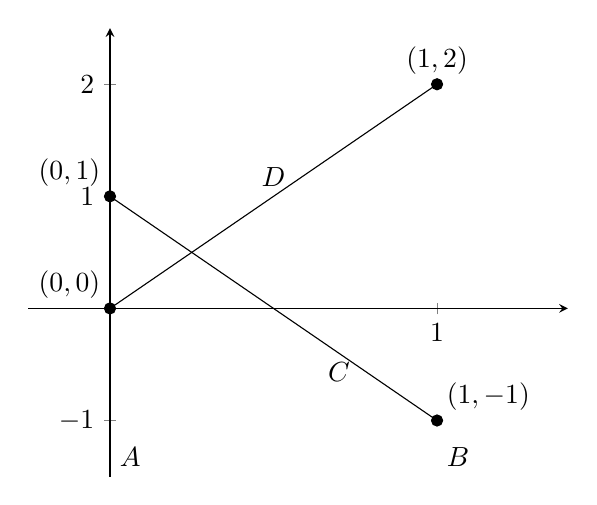
\begin{tikzpicture}
\begin{axis}[axis lines=middle, xmin=-0.25,xmax=1.4, ymin=-1.5, ymax=2.5,xtick={0,1}]
\addplot[-, mark=*]coordinates{(0,0)(1,2)}
node[pos=0,above left]{$(0,0)$}
node[pos=1,above]{$(1,2)$}
node[pos=.5,above]{$D$};

\addplot[-, mark=*]coordinates{(0,1)(1,-1)}
node[pos=0,above left]{$(0,1)$}
node[pos=1,above right]{$(1,-1)$}
node[pos=.7,below]{$C$};

\node[anchor=south west]
at ({axis cs:0,0}|-{axis description cs: 0,0}){$A$};

\node[anchor=south west]
at ({axis cs:1,0}|-{axis description cs: 0,0}){$B$};

\end{axis}
\end{tikzpicture}
\captionof{figure}{Mixed Strategy Two Lines}
   \label{F:Player 2's pure strategy D}
\end{center}   
\end{figure}

Now we can see that if Player 2 plays only D, then Player 1 does best by playing only B.
\end{itemize}

\end{itemize}

So we have this nice graph, but what does it really tell us? Although we drew lines representing each of Player 2's pure strategies, Player 1 doesn't know what Player 2 will do. Suppose Player 1 only played A, while Player 2 plays an unknown mixed strategy. Then the possible payoffs for Player 1 are 1 or 0. The more often Player 2 plays C, the more often Player 1 gets 1. So the \emph{expected payoff}\index{expected payoff} per game for a repeated game varies between 0 and 1. We can see the possible expected values as the red line on the graph in Figure \ref{F:BoldA}.

%\break

%\begin{figure}[h]
%\leavevmode
%\begin{center}
%{\scalebox{.65}{\input{graph4.pstex_t}}}
%\end{center}
%\end{figure}  
\begin{figure}
\begin{center}
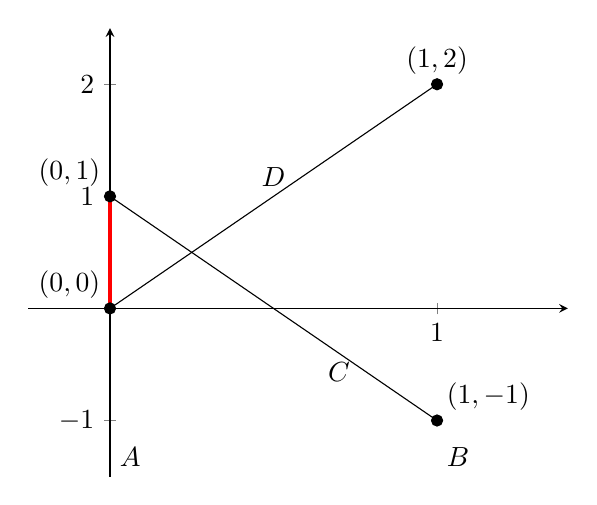
\begin{tikzpicture}
\begin{axis}[axis lines=middle, xmin=-0.25,xmax=1.4, ymin=-1.5, ymax=2.5,xtick={0,1}]
\addplot[-, mark=*]coordinates{(0,0)(1,2)}
node[pos=0,above left]{$(0,0)$}
node[pos=1,above]{$(1,2)$}
node[pos=.5,above]{$D$};

\addplot[-, mark=*]coordinates{(0,1)(1,-1)}
node[pos=0,above left]{$(0,1)$}
node[pos=1,above right]{$(1,-1)$}
node[pos=.7,below]{$C$};

\addplot[-, ultra thick, red]coordinates{(0,0)(0,1)};
%node[pos=0,above left]{$(0,1)$}
%node[pos=1,above right]{$(1,-1)$}
%node[pos=.7,below]{$C$};

\node[anchor=south west]
at ({axis cs:0,0}|-{axis description cs: 0,0}){$A$};

\node[anchor=south west]
at ({axis cs:1,0}|-{axis description cs: 0,0}){$B$};

\end{axis}
\end{tikzpicture}
\captionof{figure}{Possible expected value if Player 1 plays A}
   \label{F:BoldA}
\end{center}   
\end{figure}

Since we want to understand mixed strategies for Player 1, what would happen if Player 1 played A half the time and B half the time? In other words, what happens if $p=1/2$? Although we may not easily be able to see the exact values, we can represent the possible expected values on the graph in Figure \ref{F:BoldHalf}

%\begin{figure}[h]
%\leavevmode
%\begin{center}
%{\scalebox{.65}{\input{graph5.pstex_t}}}
%\end{center}
%\end{figure}  

\begin{figure}
\begin{center}
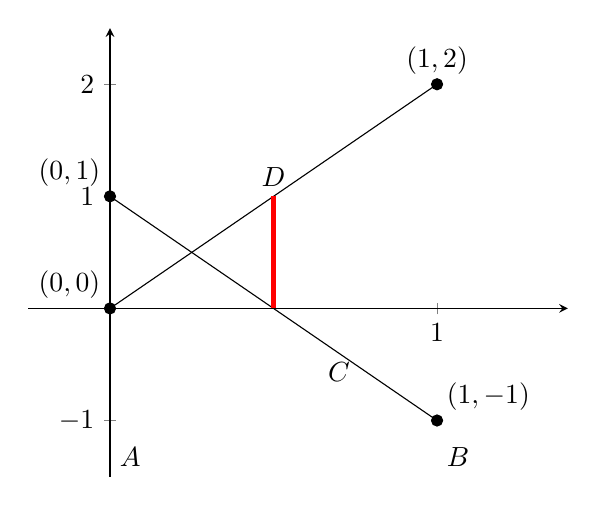
\begin{tikzpicture}
\begin{axis}[axis lines=middle, xmin=-0.25,xmax=1.4, ymin=-1.5, ymax=2.5,xtick={0,1}]
\addplot[-, mark=*]coordinates{(0,0)(1,2)}
node[pos=0,above left]{$(0,0)$}
node[pos=1,above]{$(1,2)$}
node[pos=.5,above]{$D$};

\addplot[-, mark=*]coordinates{(0,1)(1,-1)}
node[pos=0,above left]{$(0,1)$}
node[pos=1,above right]{$(1,-1)$}
node[pos=.7,below]{$C$};

\addplot[-, ultra thick, red]coordinates{(.5,0)(.5,1)};
%node[pos=0,above left]{$(0,1)$}
%node[pos=1,above right]{$(1,-1)$}
%node[pos=.7,below]{$C$};

\node[anchor=south west]
at ({axis cs:0,0}|-{axis description cs: 0,0}){$A$};

\node[anchor=south west]
at ({axis cs:1,0}|-{axis description cs: 0,0}){$B$};

\end{axis}
\end{tikzpicture}
\captionof{figure}{Player 1 plays B with probability 1/2}
   \label{F:BoldHalf}
\end{center}   
\end{figure}

Hopefully, you've begun to see that for each choice of $p$, the top line represents the highest expected value for Player 1; the bottom line represents the lowest expected value for Player 1; the area between the lines represents the possible expected values for Player 1. As we did with non-repeated games, let's look at the ``worst case scenario'' for Player 1. In other words, let's assume that Player 2 can figure out Player 1's strategy. Then Player 1 would want to \emph{maximize the minimum expected value}. Aha! This is just looking for the \emph{maximin} strategy\index{maximin strategy, repeated games}! 

Now the minimum expected value for each choice of $p$ is given by the bottom lines on the graph, shown in red in Figure \ref{F:BoldMin}.

%\begin{figure}[h]
%\leavevmode
%\begin{center}
%{\scalebox{.65}{\input{graph6.pstex_t}}}
%\end{center}
%\end{figure}  

\begin{figure}
\begin{center}
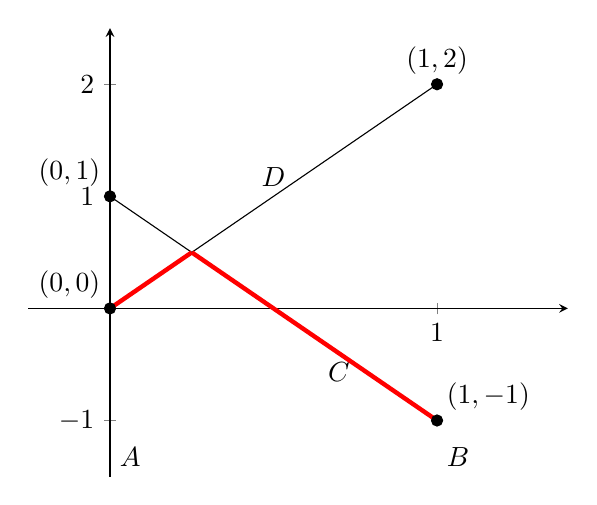
\begin{tikzpicture}
\begin{axis}[axis lines=middle, xmin=-0.25,xmax=1.4, ymin=-1.5, ymax=2.5,xtick={0,1}]
\addplot[-, mark=*]coordinates{(0,0)(1,2)}
node[pos=0,above left]{$(0,0)$}
node[pos=1,above]{$(1,2)$}
node[pos=.5,above]{$D$};

\addplot[-, mark=*]coordinates{(0,1)(1,-1)}
node[pos=0,above left]{$(0,1)$}
node[pos=1,above right]{$(1,-1)$}
node[pos=.7,below]{$C$};

\addplot[-, ultra thick, red]coordinates{(0,0)(.25,.5)};

\addplot[-, ultra thick, red]coordinates{(.25,.5)(1,-1)};
%node[pos=0,above left]{$(0,1)$}
%node[pos=1,above right]{$(1,-1)$}
%node[pos=.7,below]{$C$};

\node[anchor=south west]
at ({axis cs:0,0}|-{axis description cs: 0,0}){$A$};

\node[anchor=south west]
at ({axis cs:1,0}|-{axis description cs: 0,0}){$B$};

\end{axis}
\end{tikzpicture}
\captionof{figure}{Minimum Expected Payoff for Player 1}
   \label{F:BoldMin}
\end{center}      
\end{figure}

It should be easy to see that the \emph{maximum} of the minimum expected payoffs occurs at the intersection of the two lines.

\begin{itemize}
\item[Step 3.] Find the intersection of the two lines.
\begin{itemize}
\item[Step 3a.] Find the equation for Line C. 

This is the line passing through the points $(0, 1)$ and $(1, -1)$. It has slope $-2$ and $y$-intercept 1. Thus, it has equation $y=-2x+1$. [Although the $x$-axis represents probability $p$ and the $y$-axis represents expected payoff $m$, you are probably more comfortable solving equations--at least for the moment--in $x$ and $y$.]

\item[Step 3b.] Find the equation for Line D. 

This is the line passing through the points $(0, 0)$ and $(1, 2)$. It has slope $2$ and $y$-intercept 0. Thus, it has equation $y=2x$. 
\item[Step 3c.] Use substitution to find the point of intersection. 
\begin{eqnarray*}
2x &=&-2x+1\\
4x &=& 1\\
x&=&{1\over 4}
\end{eqnarray*}

Substituting $x={1\over 4}$ back in to either original equation, say $y=2x$, gives us $y={1\over 2}$. Thus, the point of intersection is $(1/4, 1/2)$. 
\end{itemize}

\item[Step 4.] Determine Player 1's maximin mixed strategy\index{maximin mixed strategy}. 

Recalling that the first coordinate is $p$, the probability that Player 1 plays \textbf{B}, we know that Player 1 will play B with probability 1/4, and thus, play A with probability 3/4 [$1-1/4=3/4$]. The expected payoff for Player 1 is 1/2. It is important to check back to your original intuition about the game from Exercise \ref{E:linearconjecture}. Did it seem as though Player 1 should play A more often than B?


\end{itemize}

Let's make a few important observations. First, it should be clear from the graph that Player 1 expects a payoff of 1/2 NO MATTER WHAT PLAYER 2 DOES. Furthermore, since this is a zero-sum game, we know that Player 2's expected payoff is $-1/2$. It is important to note that this graph does not give us any information about an optimal strategy for Player 2. We will see how to find a strategy for Player 2 in the following exercises. Can you think of how you might do this?
